\documentclass[11pt]{article}
\usepackage{../EllioStyle}
\usepackage{listings}
\usepackage{multicol}

\definecolor{codegreen}{rgb}{0,0.6,0}
\definecolor{codegray}{rgb}{0.5,0.5,0.5}
\definecolor{codepurple}{rgb}{0.58,0,0.82}
\definecolor{backcolour}{rgb}{0.95,0.95,0.92}

\graphicspath{ {imgs/} }

\title{Notesheet}
\author{Elliott Pryor}
\date{19 October 2022}

\lhead{Elliott Pryor}
\rhead{Notesheet}

\begin{document}
\multicols{2}

\section{Dynamics}
Generally: $\dot{x} = f(x,u), y = h(x,u)$, $x \in \reals^n, u \in \reals^m$.\\
Jacobian Linearization: given $u = u_0, x=x_0$ is a stationary point ($f(x_0, u_0) = 0$),
then $\dot{x} \approx J_{f,x}x + J_{f,u}u, y \approx J_{h,x}x + J_{h,u}u$ \\


\section{Linear Algebra}
Linear dependence $\exists \alpha_1, \dots \alpha_m$ not all zero, $\alpha_1 x_1 + \dots + \alpha_m x_m = 0$.\\
Simlarity: $B$ is similar to $A$ if $\exists Q, \, st. \, B = QAQ^{-1}$.
Columns of $Q$ are eigenvectors, B is diagonal of eigenvalues.\\
Generalized eigenvectors and Jordan: if not $n$ linearly independent eigenvectors;
solve $Av_1 = v_2$, until chain ends. \\
$rank(A) = $ \# of independent columns = size of largest-square submatrix with nonzero det.
$rank(A) + nullity(A) = $\# of columns. \\
Positive definite if any of \begin{enumerate}
    \item Every eigenvalue of $M$ is positive \textcolor{blue}{(non-negative)}
    \item All leading principal minors of $M$ are positive \textcolor{blue}{(All principal minors are non-negative)}
    \item There exists a non-singular matrix \textcolor{blue}{(matrix)} $N \in \reals^{m\times n}$ such that $M = N^TN$
\end{enumerate}
Singular Value Decomposition (SVD) is a matrix factorization technique that decomposes a matrix into three matrices:
$A = U \Sigma V^T$
where $A$ is an $m \times n$ matrix, $U$ is an $m \times m$ orthogonal matrix, 
$\Sigma$ is an $m \times n$ diagonal matrix with non-negative real numbers on the diagonal (known as singular values),
and $V$ is an $n \times n$ orthogonal matrix.
$A^TA$ has eigenvalues $\sigma_i^2$ where $\sigma_i$ are singular values of $A$.
$A^TA$ has eigenvectors $v_i$ where $v_i$ are right singular vectors of $A$.
$AA^T$ has eigenvalues $\sigma_i^2$ where $\sigma_i$ are singular values of $A$.
$AA^T$ has eigenvectors $u_i$ where $u_i$ are left singular vectors of $A$.
$A = \sum_{i=1}^r \sigma_i u_i v_i^T$ where $r = rank(A)$.
$AV = U\Sigma \implies Av_1 = \sigma_1 u_1$\\

Cayley-Hamilton: let $\Delta(\lambda) = det(A - \lambda I)$, then $\Delta(A) = 0$.\\
For any $f(A)$: $f(A) = \beta_0 I + \dots + \beta_{n-1}A^{n-1}$.
If $f$ polynomial, let $h(\lambda) = \beta_0 + \beta_1 \lambda + \dots + \beta_{n-1} \lambda ^{n-1}$,
solved from $f^{(l)}(\lambda_i) = h^{(l)}(\lambda_i)$.

Matrix exponential: $e^{At} = \sum_{k=0}^\infty \frac{1}{k!} t^k A^k$\\
$e^{A(t_1 + t_2)} = e^{At_1}e^{At_2}$, $(e^{At})^{-1} = e^{-At}$, $\frac{d}{dt} e^{At} = e^{At}A = A e^{At}$,
$e^{At} = \mathcal{L}^{-1}((sI - A)^{-1})$

\begin{center}
    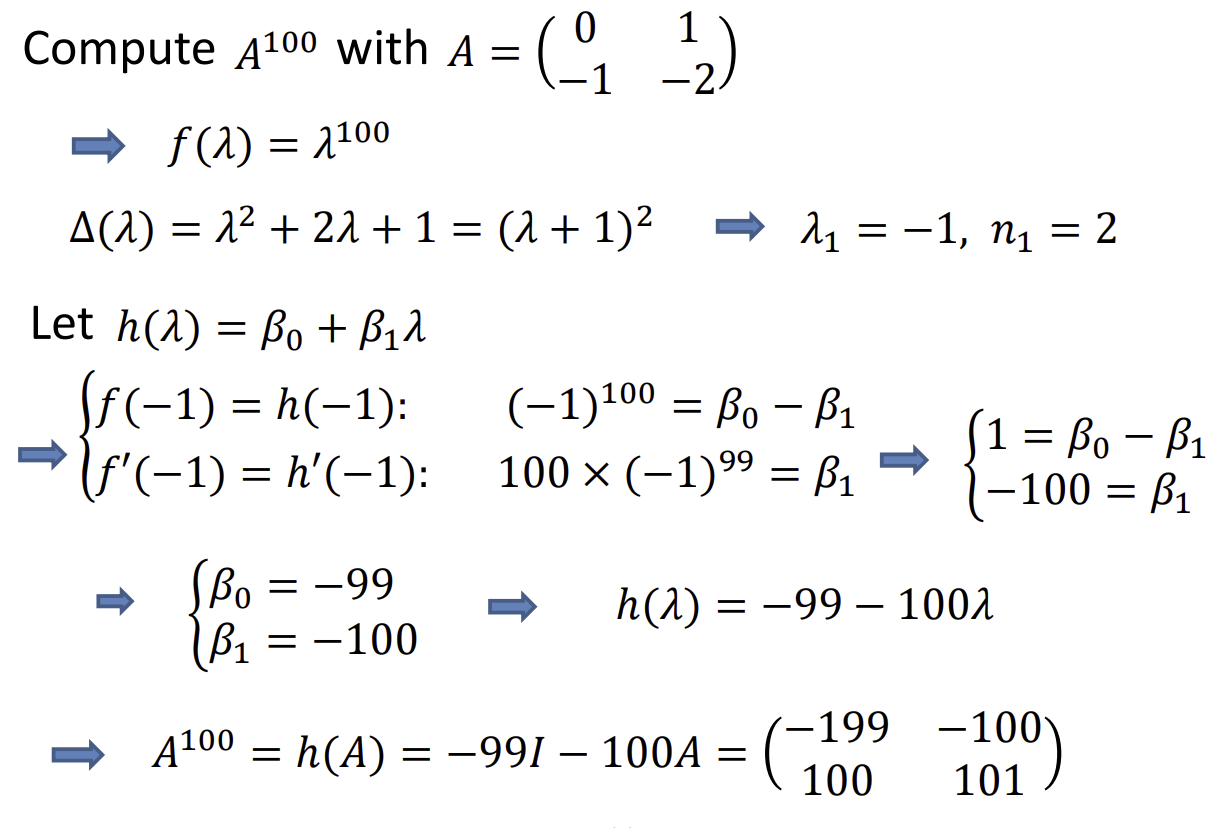
\includegraphics[width=0.9\linewidth]{cayleyhamilton.png}
\end{center}


\section{Other}

Capacitor - $i = C \frac{dv}{dt}$, Inductor: $v = L \frac{di}{dt}$, Friction $F = -k v$

\begin{center}
    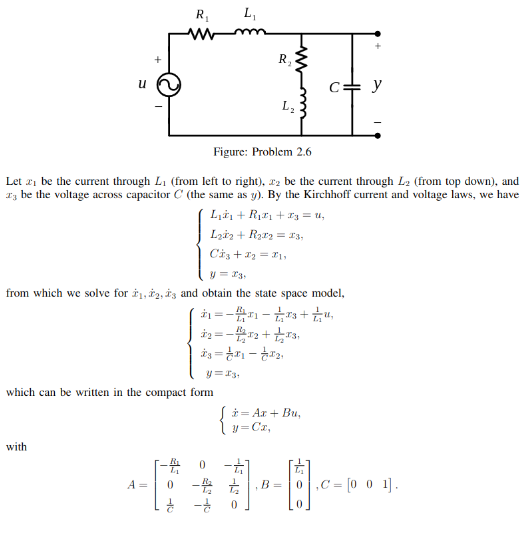
\includegraphics[width=0.99 \linewidth]{10-09-p1.png}
\end{center}

\end{document}